\section{Workflow for data quality improvement}
ARM data reprocessing to address data quality issues was
designed as an end-to-end workflow from collection of data quality
issues and concern, reprocessing for data quality improvement, review
for accuracy, versioning and archival and user notification (Figure~\ref{fig:flowchart}).
The computational workflow for reprocessing data to address data quality
issues was developed in Python programming language. The software
framework was designed for computational performance and cross-platform
compatibility. 

\begin{figure}
 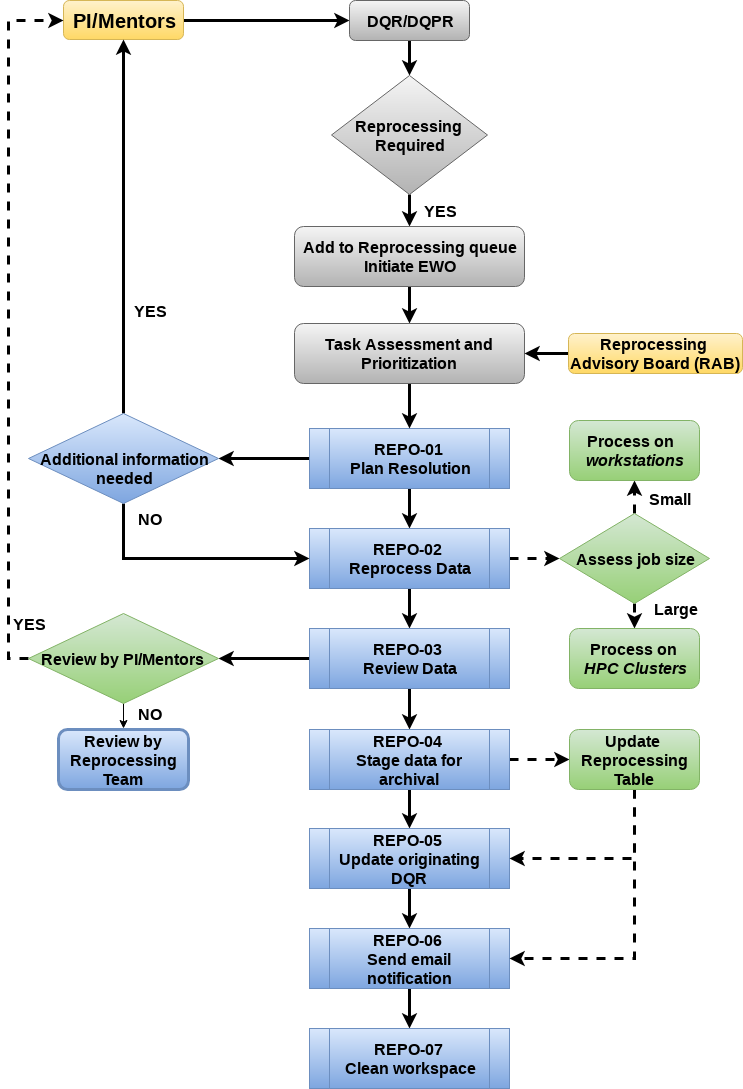
\includegraphics[width=\linewidth]{figures/reprocessing_flowchart.png}
 \caption{End-to-end workflow to reprocess data for quality improvement}
 \label{fig:flowchart}
\end{figure}

\subsection{Data Quality Reporting Tool}



\subsection{Automating data processing}
An end-to-end computational workflow was developed for data quality
improvement to address the reported data quality issue.

\subsubsection{Data staging and processing environment}
Raw data from all ARM instruments are versioned and saved in deep
archive on High Performance Storage System (HPSS) \cite{Watson_HSI_2005}
at Oak Ridge Leadership Computing Facility \cite{olcf_hpss}. An
automated process was developed to query the database for any data
quality issue based on it's unique DQRID, identify all raw data files
impacted by the issues and retrieves it from the archive. Two different
methods for data retrievals were implemented: 1) automated retrievals
using HPSS Hierarchical Storage Interface (HSI) \cite{Watson_HSI_2005}
which can be used across
most of the computational systems within ARM Data Center, however,
performs a sequential retrieval of files; and 2) a Globus Online
\cite{Foster_Globus_2011,Allen_SSD_2012} based
fast and parallel transfer mechanism suitable for large volumes of data.  

\subsubsection{Instrument data dictionaries}
Raw data from each individual instrument, which number in hundreds across
ARM facility, are all often different depending on sensors, data
characteristics and manufacturers and range from space or comma
separated ASCII, binary, hex etc. Ability to automate the processing of
datasets require a good machine readable metadata and descriptors for
each instrument. Traditional processing workflows were custom
designed for individual instruments and thus lead to rigid workflow that
required custom developments to address any quality issues. As part of
automated workflow, detailed data dictionaries were designed and saved
in machine readable JSON formats that allowed for automated processing
of data. Data dictionary encodes the format of raw instrument data,
numerical procedure to calculated derived variables, and ARM standard
variable names and units (Figure~\ref{fig:met_dict}). Data dictionaries
also captures any historical change or update to instrument data format
or observations. Figure~\ref{fig:met_dict} shows an example data
dictionary for surface meteorology (MET) instruments the contains the
column-wise mapping of data in raw ASCII format, expected data type,
units and names for standard primary and derived variables.
Library of comprehensive data dictionaries are the
critical to enable automation of data quality control and improvements
at scale across large observational facility like ARM. 

\begin{figure}
 \centering
 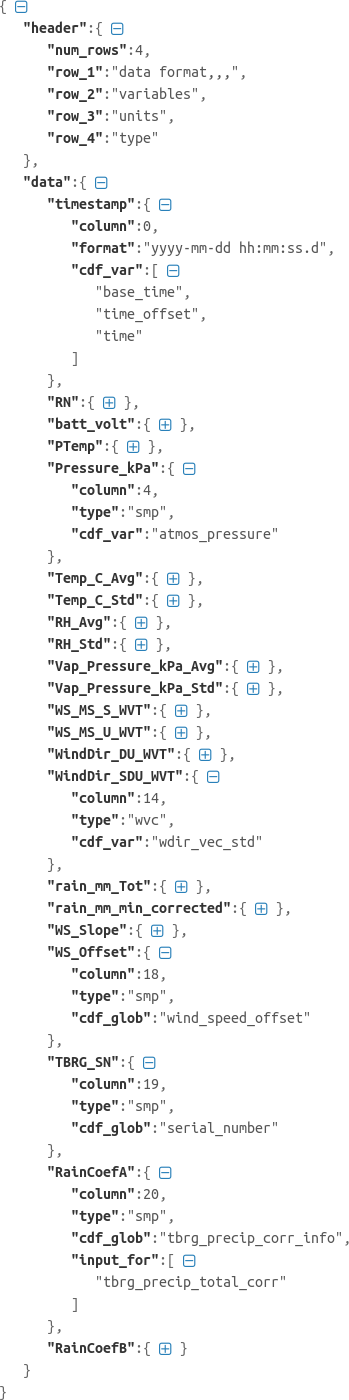
\includegraphics[width=0.6\linewidth]{figures/met_dict.png}
 \caption{Data dictionary for MET instrument contains information about
	 the raw data format, standard variable names, units, variable dependencies
	 and other metadata in a JSON format.}
 \label{fig:met_dict}
\end{figure}

\subsubsection{Symbolic equations processing}
As part of automated data processing framework, a capability for
symbolic equation processing was developed using Python \texttt{SymPy}
\cite{sympy}. Equations for calculating any primary or derived are
derived from instrument data dictionaries or provided by instrument
experts as part of the associated DQR. Equations provided with DQRs are
given precedence over ones from data dictionaries. Framework was
designed to ensure the correctness of associated variables to be
processed for any given data stream. When solving system or set of
equations, the framework was designed to detect and handle and variable
dependence and/or conflict. If primary variable is changed as part of
a data quality issue, all dependent derived variables were recalculated
to ensure correctness of the entire data stream as part of the processing.
Framework was implemented and tested for a range scenarios experienced
within ARM datasets for correctness before being deployed in an
operation. Ability to process symbolic allowed for automation of data
improvement workflow, avoid need for any custom development and
processing by an analyst.

\subsubsection{High performance computing for big data processing}
For efficient processing of large volumes of data, capability for
parallel data processing was developed. Most ARM time series data are
packaged in one or more files per day allowing for their simultaneous
processing in a embarrassingly parallel fashion. Two parallel processing
framework were implemented within the Python based software framework,
to allow for use and execution on small shared memory computing
environment to medium to large scale distributed memory computing
environments. For shared memory environment, parallelism was achieved
using Python \texttt{multiprocessing} while Python \texttt{Dask}
\cite{dask} was used for parallel data processing on distributed memory
compute clusters. For task requiring processing for large volume of
data, data transfers times are significant and system was designed to
overlap data staging and processing to allow processing of data as they
become available.

\subsubsection{Data review}
Review of the processing performed on the data is critical to ensure
that the actions undertaken accurately and satisfactorily addressed the
data quality issues reported in the associated DQR.
A formal and comprehensive data review was conducted for all data
processed, comparing old and new data products to identify variables
affected, compute statistics for change and generate interactive plots
to visualize the data. Data review was one of the only step that was
designed to require a human intervention, in form of review either by
the instrument expert of the data analyst. While the workflow was
designed for automation, the free-form description section of the DQR
may at times contain special instruction or information that may have been missed by the
automation workflow. Data review was designed to provide the oversight
to ensure the accuracy of the data. If the data review check is
successful, it triggers the execution of the rest of the workflow,
however in case an issue is identified the processing task is
assigned to a data analyst. 






\section{Data versioning and archival}
Once an updated version of data with improved data quality is prepared,
it is formally assigned a version for tracking. However, versioning for
complex data like those in ARM pose unique challenges which led to
development of new data versioning system deployed across the facility
\cite{Macduff_2014}. Data reprocessing to data quality improvement,
however, at times leads to versioning conflict scenarios. Versioning
module of the workflow extends the current versioning scheme
\cite{Macduff_2014}.

Standard ARM filename and versioning includes site, facility, instrument
and start time of observation time series in filename. However, length
of time series contained within the file are not reflected in the
filename and thus creating conflict when data are reprocessed.
ARM file standards also allow for any arbitrary number of files within a day
during a real time processing, while reprocessing for data quality
improvements on past data often create longer continuous time series and
thus few files. To identify and address these conflicts all affected
files (old and new) were checked for the start and end of the time
series. In particular following scenarios occur frequently: 

\begin{enumerate}
 \item Near-real-time processing may create multiple partial day files
 within a day (ex. fileA.v0: 00:00:00--12:00:00 and fileB.v0:
 12:00:01--24:00:00) if the observations from the remote instruments as
 observations arrive at the data center in chunks 
 due to network bandwidth or some other issue. However, the reprocessing
 for the data may create a single file with continuous time series 
 (ex. fileA: 00:00:00--24:00:00).
 While the filename of the newly created file would be same as one of
 the existing files and will be assigned the correct incremental
 version number (ex. fileA.v1: 00:00:00--24:00:00), the rest of the 
 old files (ex. fileB: 12:00:01--24:00:00) from the day would identified
 and marked to be obsolete and marked unavailable in future.
 \item File versioning tracks the versions of a filename, but during the
 process of reprocessing it's possible for new filenames to be created.
 For example, if data in original fileA.v0: 01:00:00--24:00:00 was
 reprocessed to correct the quality issue during first hour of the day
 that was excluded for the original processing, a new fileB.v0:
 00:00:00--24:00:00 will be created and while no filename conflict occur
 with fileA.v0, fileA.v0 must be deleted and marked unavailable to avoid
 conflicting time series data.
\end{enumerate}

Once the file has been assigned the correct name and version, it is
archived in the deep archive on HPSS and a copy is placed on new data
cache while the older data are made unavailable. ARM's comprehensive
database of all file holdings are also updated as a part of the archival step.



\section{Data provenance tracking}
Accuracy and reproducibility is essential component of sound and
reliable scientific research and analysis. Capturing rigorous provenance
information at every step of data life cycle is critical to allow
reproducible science. Data reprocessing workflow for data quality
improvement modifies the data from its original version and its
paramount that the provenance of the data be comprehensively captured.
While the technical details of the data quality issue and its
implication are detailed in the DQR, the reprocessing workflow was
designed to log details of every step of the processing including
versioned filenames of each data file processed, variables recalculated,
symbolic equations applied for processing, softwares including versions
used in processing, computing systems used etc. A subset of provenance
information relevant for scientific users of the data was also appended
to the DQR, that are distributed along with the data. 



\section{Communicating data quality changes}
Clear and timely communication of the data quality changes are important
for scientific users. While the description of data quality issues and
remedial actions taken to address them are available publicly as part of
the DQR associated with the data, they may not reach the data users who
have downloaded and used the data in the past. We utilized the database
of historical data download history to identify all users who have
downloaded the data affected as part of a data reprocessing and
communicate via an automated email to them a summary of changes to the
data to inform them of the change. The email notifications are also sent
to instrument principal investigators, and developer of Value Added
Product that are using the data product and thus may be affected by the
change in the data quality.





